%%%%%%%%%%%%%%%%%%%%%%%%%%%%%%%%%%%%%%STARt PREAMBLE
\documentclass{article}

%Required: You must have these
\usepackage{Sweave}
\usepackage{graphicx}
\usepackage{tabularx}
\usepackage{hyperref}
\usepackage{natbib}
\usepackage{pdflscape}
\usepackage{array}
\usepackage{authblk}
\usepackage{gensymb}
\usepackage{amsmath}
%\usepackage[backend=bibtex]{biblatex}
%Strongly recommended
 %put your figures in one place
%\SweaveOpts{prefix.string=figures/, eps=FALSE} 
%you'll want these for pretty captioning
\usepackage[small]{caption}

\setkeys{Gin}{width=0.8\textwidth} %make the figs 50 perc textwidth
\setlength{\captionmargin}{30pt}
\setlength{\abovecaptionskip}{10pt}
\setlength{\belowcaptionskip}{10pt}
% manual for caption http://www.dd.chalmers.se/latex/Docs/PDF/caption.pdf

%Optional: I like to muck with my margins and spacing in ways that LaTeX frowns on
%Here's how to do that
\topmargin -1.5cm  
\oddsidemargin -0.04cm 
\evensidemargin -0.04cm % same as oddsidemargin but for left-hand pages
\textwidth 16.59cm
\textheight 21.94cm 
%\pagestyle{empty}  % Uncomment if don't want page numbers
\parskip 7.2pt   % sets spacing between paragraphs
%\renewcommand{\baselinestretch}{1.5} 	% Uncomment for 1.5 spacing between lines
\parindent 0pt% sets leading space for paragraphs
\usepackage{setspace}
%\doublespacing
\renewcommand{\baselinestretch}{1}
\usepackage{lineno}
 
%%%%%%%%%%%%%%%%%%%%%%%%%%%%%%%%%%%%%%END PREAMBLE 

%Start of the document
\begin{document}

%\SweaveOpts{concordance=FALSE}
\Sconcordance{concordance:bayes4cons_doc.tex:bayes4cons_doc.Rnw:1 310 1}


\bibliographystyle{bibstyles/amnat.bst}
\title{Benefits of Bayesian Modelling Approaches For Conservation Science Under Climate Change} 
\author[1,a]{A.K. Ettinger}
\author[2]{H. Eyster}
\author[3]{D. Loughnan}
\author[3]{X. Wang}
\author[3]{E.M. Wolkovich}
\author[3]{M. Auger-Methe}
\author[4]{R. Zenil-Ferguson}
\author[5]{V. Leos Barajas}
\author[6]{Leithen M'Gonigle}
\author[6]{Hanna Jackson}
\author[7]{Others from Symposium working group?}


\affil[1]{The Nature Conservancy,Seattle, Washington, USA}
\affil[2]{TNC}
\affil[3]{UBC}
\affil[4]{UKY}
\affil[5]{University of Toronto}
\affil[6]{SFU}
\affil[7]{Multiple other institutions?}


\affil[a]{Corresponding author; email: ailene.ettinger@tnc.org; mailing address: 74 Wall Street. Seattle, WA 98121, USA }

\date{\today}
\maketitle 
\textbf{Author contributions}: All authors conceived of this manuscript, which began through conversations at a Bayesian Generative Modelling Symposium at University of British Columbia in 2024; AKE led the writing of the manuscript, all authors contributed portions of text and revised the manuscript.

\textbf{Data Accessibility} 

\textbf{Running title} 

\textbf{Key words} 


\textbf{Paper type} \textit{Perspective} in \href{https://conbio.onlinelibrary.wiley.com/hub/journal/25784854/homepage/author-guidelines}{Conservation Science and Practice} 

\textbf{Focal Audience} Conservation biologists and other scientists who contribute to or would like to influence conservation and environmental policy (e.g., iPCC, IUCN)

%%%%%%%%%%%%%%%%%%%%%%%%%%%%%%%%%%%%%%%%%%%%%%%%%%%

%%%%%%%%%%%%%%%%%%%%%%%%%%%%%%%%%%%%%%%%%%%%%%%%%%%

%\linenumbers

\section*{Abstract} 



\newpage
\section* {Introduction}

\par Conservation science in the 21st century seeks to address the dual crises of  climate change and rapid biodiversity loss. These are problems that require urgent action globally, as loss of earth's biodiversity and its benefits are accelerating \citep{brondizio2019assessing, ripple2017extinction,tittensor2014mid}. Could be something like: Climate change has added complexity to conservation biology's traditional goal of conserving biodiversity. Because climate change both affects and is affected by conservation actions, how to integrate it fully into the discipline and its resolutions and goals (Convention on Biological...) is a major challenge. One major approach has been to include global climate change mitigation assesment and effort, such as through the concept of `natural climate solutions' (NCS) \citep{ellis2024principles}. NCS are intentional human actions (or `NCS pathways') that protect, restore, and improve management of forests, wetlands, grasslands, oceans, and agricultural lands to mitigate climate change \citep{griscom2017natural}.

\par The need for robust and usable conservation science under climate change is necessary at scales ranging from local to global. For example, preserve managers seek guidance about how to best steward natural resources for climate resilience \citep{Nadeau2015}, international climate policy relies on scientific data and publications for systematic observation of climate systems and impacts to people. \cite{ipcc2007}. Developing the evidence base for urgent climate and biodiversity questions often requires synthesizing multiple data sources and incomplete datasets, given the complex social ecological systems in which many conservation science problems are grounded. Thus, a critical part of building the evidence base is ensuring reproducibility and transparency, including clear communication of uncertainty \citep{ellis2024principles,ipcc2007}. %DLJuly30: I know this is a commonly used phrase, but is it necessary to introduce this complex framework? Could we not just say "complex ecological systems"?

\par Bayesian data analysis provides a framework and approaches that supports these needs of conservation science in the 21st century. Bayesian approaches facilitate synthesis of multiple sources of data to update probabilities of focal outcomes of interest after examining new data (e.g., priors, see Box 1). Bayesian methods are well-suited to decision making, as they moving beyond strict null-hypothesis testing to
%whereas frequentist inference estimates the probability that the observed data occurred given a particular hypothesis (P(Y|H)),Bayesian inference  
provide a quantitative measure of the probability of a hypothesis being true given the available data. % (P(H|Y)). Further, Bayesian approaches provide stratightforward approaches to propagate uncertainty through posterior distirbutions. 
Some fields within conservation biology and natural resource management have adopted Bayesian methods (e.g., wildlife mark and recapture models or occupancy models \citep{Kery2011}, fisheries\citep{Doll2018}), but historically they have not been widely used in conservation biology (REF FIGURE).

\subsection*{Aim} We aim to highlight features of Bayesian approaches that are well-suited to conservation science to practitioners who may be unfamiliar with Bayesian methods, and hope to accelerate more widespread adoption of Bayesian data analytical approaches in conservation. We believe that, with more widespread adoption, these approaches could enhance progress of conservation science. We start by describing some of the benefits of using Bayesian methods to address conservation science questions. We show that Bayesian approaches have been steadily increasing in ecology and natural resource management, highlighting that the time is right for more widespread use and integration into conservation science, policy, and practice. We also summarize Bayesian workflows, provide example code and analyses through two/three case studies relevant to current conservation problems, and share resources and a glossary that we hope will make Bayesian methods more approachable to those who have not used them before.
\section* {Benefits for Conservation Science}
\subsection*{Powerful and flexible modelling approaches}
\par Ecological data are often non-normal, `unbalanced' and nested within hierarchical or non-hierarchical groupings that are non-independent (e.g., species or other groupings related to ecolutionary history/genetics, spatial clustering such as plots or sites, or temporal clustering such as day or year). Bayesian modelling approaches are well-suited to these data, given their flexibility and power to provide robust estimates under a wide range of conditions (e.g., Case Study 1). . %DLJuly30: I think you could be more explicit here: "Bayesian modelling approaches address many of these limitations, while being flexible..."
\par In addition, conservation biologists are often particularly interested in species with small populations, since these are often the ones most at risk of extinction, or ones that are poorly understood \citep{stinchcombe2002influence}. Bayesian methods,  do not rely on asymptotic behavior (as frequentist statistics due \citep{mcneish2016using}) and so are better able to accommodate small sample sizes. However, these methods still require care when working with small sample sizes, because priors can matter more. This is also an opportunity to include the full gamut of prior knowledge from many sources that may not typically be included in quantitative analyses. %DLJuly30: Do we need to introduce the topic of priors here or just that Bayesian approaches allow you to incorporate prior knowledge. If we do want to discuss priors, are we assuming the reader knows what priors are or citing box 1 here?  \citep{mcneish2016using}. See Case Study 3.

\par Conservation often requires putting species in easily-interpretable conservation status categories to inform decision making \citep{brooks2008quantifying}. For example, conservation might be prioritized for species declining `rapidly' versus `moderately.' These discrete categories require information about when a species' population has passed a particular threshold, and Bayesian approaches are ``natural for quantifying, in the form of a probability, the support provided by the data" for whether a species has surpassed a given threshold  \citep{brooks2008quantifying}. 

\subsection*{Frameworks for integrating multiple data sources}
\par Conservation problems are complex and addressing them, especially in the era of climate change, requires integrating social, economic, biological, and physical information to provide the evidence base upon which decisions can be made. Conservation evidence comes in many forms, including from quantitative studies, community knowledge, expert knowledge, traditional ecological knowledge, and others. Conservation decision-making requires integrating these multiple sources of information to provide an evidence base upon which decisions can be grounded \citep{stern2022interweaving}. Bayesian methods enable two fruitful avenues for such integration. First, information can be amalgamated into Bayesian Belief Networks \citep{marcot2001using,newton2007bayesian}. Second, extant information can be used to inform prior distributions \citep{o2008informed}. %DLJuly30: It sounds like you are introducing two major concepts, but the term "Bayesian Belief Networks" is never used again. I think more elaboration is needed to help the reader make the link with what is discussed below.

\subsection*{Moving beyond null hypothesis testing and $\alpha <0.05$ }
\par Conservation scientists often need to compare outcomes from current `business-as-usual' approaches to new alternatives. For example, conservation scientists might be interested in deciding whether an alternative practice produces the same results as current practice. 
The need to test new approaches, coupled with the fact that ecosystems are dynamic and often yield unexpected behaviors \citep{Levin2012,Gross2013}, have led to practices of adaptive management in conservation \citep{holling1978adaptive} (Fig. \ref{fig:workflow}). %Yet frequentist statistical frameworks rarely provide information necessary to adequately inform adaptive management \citep{prato2005bayesian}.  Specifically, frequentist statistics' incapacity to compare support for a variety of hypotheses \citep[including a `null' hypothesis;][]{Zyl2018} prevents this method from informing what interventions will most likely bring about conservation gains \citep{prato2005bayesian}. For example, in its submission process, leading conservation journal \textit{Conservation Biology} requires that authors recognize that, `8. ensured you have not misinterpreted statistical nonsignificance as no effect if a frequentist approach was used (absence of evidence is not evidence of absence)?' 
Bayesian analysis is beneficial in that it is flexible enough to allow comparison of support for a variety of hypotheses or interventions, including a null hypothesis \citep{Zyl2018}. On other words, Bayesian approaches facilitate comparing, for example, which interventions will most likely bring about conservation gains \citep{prato2005bayesian}, or whether the current versus alternative management practices produce similar results \citep{gallistel2009importance}.

\par Null hypothesis significance testing and conventions of rejecting the null hypohtesis when $\alpha <0.05$ have long been dominant in conservation biology, as in ecology and related biological fields \citep[e.g., ecotoxicaology][]{erickson2020moving}. mP-value-focused conventions are becoming less prevalent, but many biologists are unsure of alternative ways to analyse and interpret their data \citep{halsey2019reign}. Bayesian approaches and workflows offer an alternative framework,and are not bound by conventions of $p<0.05$. Add more here i think....
%DLJuly30: I agree, I think we do need a clear discussion of what the alternative metrics are that a Bayesian analysis provides. 
\subsection*{Integrated appraoches for quantifying and propagating uncertainty} 
\par Bayesian analyses are particularly useful for decision-making because they are adept at integrating not only a range of information types, but also the uncertainty associated with these information types \citep[e.g.,][]{stern2022interweaving}. The integration of multiple datasets required by many conservation problems in turn necessitates quantifying and sometimes propagating uncertainty across multiple sources and/or multiple modeling steps (see Case Study 2). Bayesian approaches enable straightforward quantification and  propagation of  uncertainty, including for some conservation problems that can require analyses for which frequentist statistics are unable to compute the associated uncertainties \citep{bolker2009a,bates2006r}, and for which the intuitive interpretation matches the technical definition, yielding interpretable results, particularly for non-statistician colleagues and decision-makers \citep{fornacon2021bayesian}. 
\par Moreover, Bayesian methods enable uncertainty to be propagated through multiple analyses, ensuring that end results represent the full uncertainty of the process under study. \citep{draper1995assessment,gilbert2023propagating,Eyster2022,Saunders2019}. For example, using Bayesian methods, one can calculate the abundance of birds in different types of management landscapes such as traditional agriculture and perennial polycultures, and then propagate the uncertainty associated with those abundances into a downstream analysis to test whether the bird communities in the alternative perennial polyculture landscape are maintained simply as an ecological sink \citep{Eyster2022}. 

\section* {Increasing use of Bayesian approaches}
\par Use of Bayesian approaches varies across ecological fields and systems, but is generally increasing (Fig. \ref{fig:consbaystrend}). The variation across fields is notable, with more widespread use in fisheries and wildlife biology, and less in forestry  (Fig. \ref{fig:consbaystrend}).

\par  Though Bayesian methods are increasing, the are not standard, widely used approaches that are well-integrated into global systems of conservation and climate science, policy and practice (e.g., IPCC, IUCN). For example, IPCC-described methods for uncertainty propogation do not include Bayesian approaches \citep{ipcc2007}, though they offer straightforward implementation (Case Study 2).
%From Lizzie: IUCN `Rules of Procedure’ (download here) are pretty vague on uncertainty (and have two types at least: Uncertainty in the data and uncertainty in taxonomic). I think our relevant interest in the IUCN goal is to get to ‘Direction of current population trend (stable, increasing, decreasing, unknown)’ and there are actually are some papers about what to do about uncertainty in this for the IUCN. One well-cited one is: Making Consistent IUCN Classifications under Uncertainty (2000, JSTOR link), which I think basically advocated fuzzy numbers (but I did not read closely; this paper seems to have led to the RAMAS software). There’s a literature from this citation including a Bayesian network (Use of a Bayesian network for Red Listing under uncertainty, 2010) that someone could dig into a little more? See also: JARA: ‘Just Another Red-List Assessment’
\section* {Case Studies}
\subsection*{Case Stufy 1: Robust estimates of trends in species or populations of concern}
\par In some cases, Bayesian approaches can lead to importantly different conclusions than common Fisherian approaches, such as null hypothesis testing citep{wade2000bayesian}. Consider, for example, sampling five populations of a species across its range---from north to south---to monitor for changes in the population size with climate change. After collecting data for ten years, a traditional null hypothesis testing approach to analyzing the data, using the common Type I error value ($\alpha$) of 0.05 would find changes in only two of the populations---the furthest north population, which appears to be increasing, and the second furthest north population, also increasing. The three other populations are not significantly changing under this approach (Fig. \ref{fig:nht} left). In contrast, a Bayesian approach (using weakly informative priors centered at zero, all code provided in supplement) would likely focus on the posteriors, where small differences in the variance do not appear so different  (Fig. \ref{fig:nht} right). Here, a clear trend emerges where trends in population correlate with position in range---with the most northern population increasing the most and the most southern population decreasing the most. This pattern across the range is the type predicted by climate change and may be missed with a classic Fisherian approach (combining null hypothesis testing with threshold values for `significance'), leading to potential very difference conservation and management decisions. % EMW says: We could also add (1) more details on the simulations (the variance in the underlying model increases going from north to south, which is expected for smaller population sizes), (2) point out 10 years is often more years than we have; though I think there is enough text already. 


\subsection*{Case Study 2: Incorporating and propagating uncertainty}
\par We simulate flux data from a field study quantifying greenhouse gas fluxes (methane, carbon dioxide) s in peatlands with and without grazing in Ecuador (Sanchez et al) to show how Bayesian approaches can be used to propoagate uncertainty in a straightforward way. 

\begin{itemize}
\item carbon Mitigation= flux X extent, Fig. \ref{fig:ncs}
\item uncertainty propogation using posterior
\item see \href{https://github.com/AileneKane/bayes4cons/tree/main/analyses/ncs.R}{https://github.com/AileneKane/bayes4cons/tree/main/analyses/ncs.R}
\end{itemize}

\subsection*{Case Study 3: State-space model and priors example}

\par We demonstratte use of priors via a population model, described in Auger-Methe et al 2021 and based on Jamieson and Brooks (2004) and Dennis and Taper (1994). This is a simple population model with density dependence, made up of process and observation components, as described at \href{https://github.com/AileneKane/bayes4cons/blob/main/analyses/SSM.Rmd}{https://github.com/AileneKane/bayes4cons/blob/main/analyses/SSM.Rmd}

\par In this scenario, we have re-introduced 10 adult females and some 10 adult males from an extirpated species in 2003 in a conservation area, and we are monitoring their growth for the past 20 years to see if they have reached carrying capacity and what is that carrying capacity.

\par This is a species that has a long life span (e.g. 20+ years) and creates long term pairs  that can produce maximum 2 offspring when in good conditions, and therefore could be able to almost double in size ever year. Here the conservation area does not allow the animal to fulfill it's full growth ($\beta_0 = 1.3$). From a repeated assessments of the efficiency of the line transect in early years, when all of the re-introduce animals were individually marked, we know that we can miss many individuals and have estimated the $\sigma_o = 10$.

\par As for most population of this species the birth rate, which is the main source of biological stochasticity, vary by less than 5%.

\par When we fit the model with vague priors, there are many warnings, indicating the model is problematic. However, when we use knowledge gained from previous studies of species' biology to inform priors, we are able to fit models.
%DLJuly30: I think case study 3 makes the most sense as a vignette---there is a lot of ecology for the background and to explain what the priors are. As a reader, I would want an explanation for what the warnings mean and how they inform the process. I also think if our goal is to emphasize prior selection, we need to be more explicit in explaining what the vague priors are and what kinds of knowledge was needed to develop informative priors.

\section* {A future with more widespread use of Bayesian modelling in Conservation}
\begin{itemize}
\item Implementing Bayesian modelling is easier than ever before! Computational resources (add some details)- are getting easier and should continue getting easier to develop, test, and refine models that represent focal systems and are able to address relevant questions)
\item Urgency and complexity of problems and systems requires flexible, powerful modelling appraoches 
\item We envision a future in which conservation and ecology students (undegraduate and graduate levels) receive statistical training to provide strong foundations in Bayesian statistics. Many introductory statistics classes focus on t-tests and linear regressions, which are often not appropriate for ecological datasets. It doesn't have to be this way! 
\item IPCC and other global institutions should include guidelines for Bayesian approaches increasingly used by ecologists ( Fig. \ref{fig:consbaystrend}), as NCS gets integrated into the climate/biophysical analyses that dominated early IPCC work.
\end{itemize}

\par 
\section* {Box 1: Defining Bayesian Analysis (i.e., Inference and Workflow)}

\begin{enumerate}
\item Define what it is: 2-3 sentences
\begin{itemize}
\item Bayesian methods—provides a quantitative measure of the probability that a hypothesis is true using available data
\item Bayesian methods—bring prior knowledge together with the sample data
\item Does not assume that parameters are the fixed or true quantities
\item Bayesian analysis can be formulated in a variety of different ways (Lee, 2011).
\end{itemize}
\item Brief discussion of equation: 2 sentences
\begin{itemize}
\item Bayesian methods use Bayes' Theorem (eqn. 1) to combine our prior knowledge of a system with the available data to estimate the probability of an event. 
\item P(A|B) = f(B|A)(A)/P(B)
\end{itemize}
\item Three components of Bayesian: point form list
\begin{itemize}
\item Posterior distribution (P(A|B)): used to update the prior using the likelihood
\item Likelihood ( f(B|A)): function of how likely te response variable is given the data
\item Prior ((A)): pre-existing information about the hypothesis—data from pilot studies or previous experiments, knowledge from experts or the literature—reflect the uncertainty within the system
\end{itemize}
\item How to interpret the results 2-3 sentences
\begin{itemize}
\item Bayesian methods—cares about credible interval, prior, posterior
\item Since inferences are probabilistic—can perform simulations using the density distributions of their parameters and make stronger inference of models predictive uncertainty
\end{itemize}
\end{enumerate}


% Inference in frequentist statistics can take many forms, but here we focus on the most dominant incarnation, which entails testing the significance of a null hypothesis given data, measured with a p-value \citep{Zyl2018}. Bayesian analysis can be formulated in a variety of different ways (Lee, 2011). Frequentist methods have previously dominated ecological analyses.
% \begin{itemize}
% \item Frequentist methods—that rely on the frequency of an event's occurrence in a sample dataset given a particular hypothesis to estimate its probability.
% \item Bayesian methods—provides a quantitative measure of the probability that a hypothesis is true using available data
% \item Frequentist methods—only make use of the sample data
% \item Bayesian methods—bring prior knowledge together with the sample data
% \item Frequentist methods—parameters  are considered to be estimates of fixed
% \item Bayesian methods—model parameters are treated as random variables
% \item Frequentist methods—cares about p-value, significance, confidence interval
% \item Bayesian methods—cares about credible interval, prior, posterior
% \end{itemize}
% Bayesian methods use Bayes' Theorem (eqn. 1) to combine our prior knowledge of a system with the available data to estimate the probability of an event. 
% Does not assume that parameters are the fixed or true quantities
% Since inferences are probabilistic—can perform simulations using the density distributions of their parameters and make stronger inference of models predictive uncertainty
% P(A|B) = f(B|A)(A)/P(B)
% \par Three components:
% \begin{itemize}
% \item Posterior distribution (P(A|B)): used to update the prior using the likelihood
% \item Likelihood ( f(B|A)): function of how likely te response variable is given the data
% \item Prior ((A)): pre-existing information about the hypothesis—data from pilot studies or previous experiments, knowledge from experts or the literature—reflect the uncertainty within the system
% \end{itemize}
% \par Bayesian modeling is an iterative process: analyses may start with insufficient knowledge and data but use experiments to inform priors, and uses model checking to test key assumptions and our understanding of the data generating process.
% \par General bayesian workflow (Fig. \ref{fig:workflow})
% \begin{itemize}
% \item Simulate data based on priors and initial model specification 
% \item Collect data
% \item Model construction and testing
% \item Prior predictive checks→Fit model to data
% \item Posterior predictive checks
% \item Summarize posteriors
% \item Report results to targeted audiences
% \end{itemize}
% 


\section* {Box 2: Resources to Get Started}
\underline{Priors}
\par Default priors. Chosen without critical thought or evaluation. Fear of being too subjective. Defending prior choice promotes good statistical inference
\par Resources on priors: 

\begin{itemize}
\item Banner et al. 2020 https://besjournals.onlinelibrary.wiley.com/doi/full/10.1111/2041-210X.13407 
\end{itemize}

\par Other resources:
\begin{itemize}
\item A guide to Bayesian model checking for ecologists \citep{conn2018guide}
\item Gentle Introduction to Bayesian statistics \citep{van2014gentle}
\href{https://www.ncbi.nlm.nih.gov/pmc/articles/PMC4158865/}{https://www.ncbi.nlm.nih.gov/pmc/articles/PMC4158865/}
\item Bayesian model selection for ecologists. \citep{hooten2015guide}
 \href{https://doi.org/10.1890/14-0661.1}{https://doi.org/10.1890/14-0661.1}
\item Bayesian Inference for ecologists. \citep{elis2004}
\item Why becoming Bayesian? \citep{clark2005environmental}
 \href{https://doi.org/10.1111/j.1461-0248.2004.00702.x}{https://doi.org/10.1111/j.1461-0248.2004.00702.x}
\item Bayesian Workflow \citep{gelman2020bayesia}

\end{itemize}
 


\bibliography{conslib.bib}

\section* {Figures}
 \begin{figure}[h]
\centering
 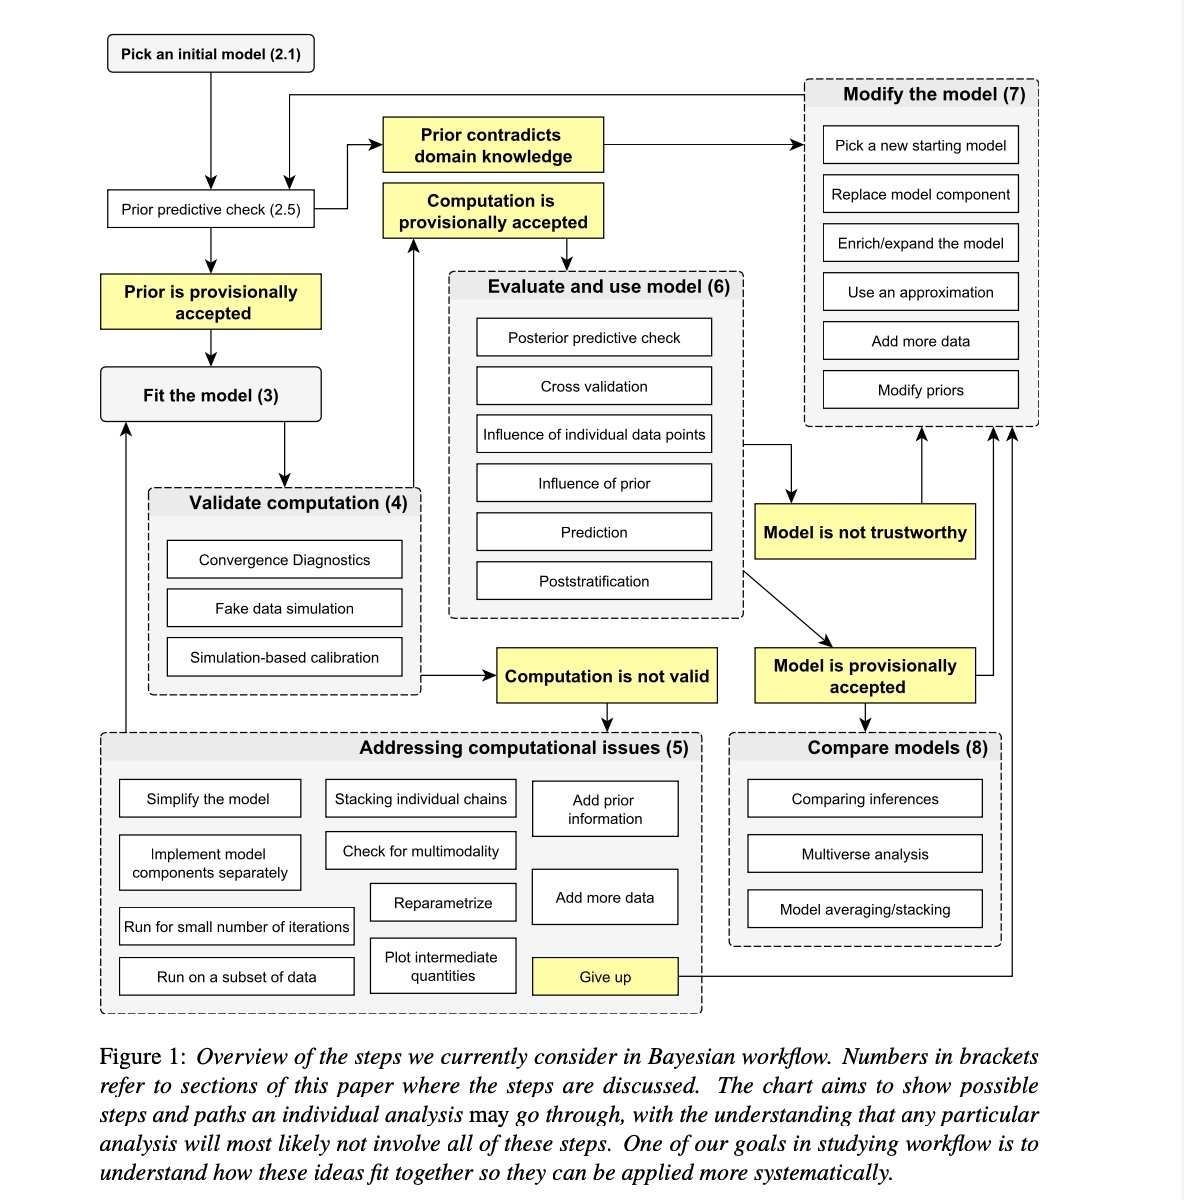
\includegraphics[width=0.75\textwidth]{../figs/BayesianWorkflowfromGelman2020.jpg}
  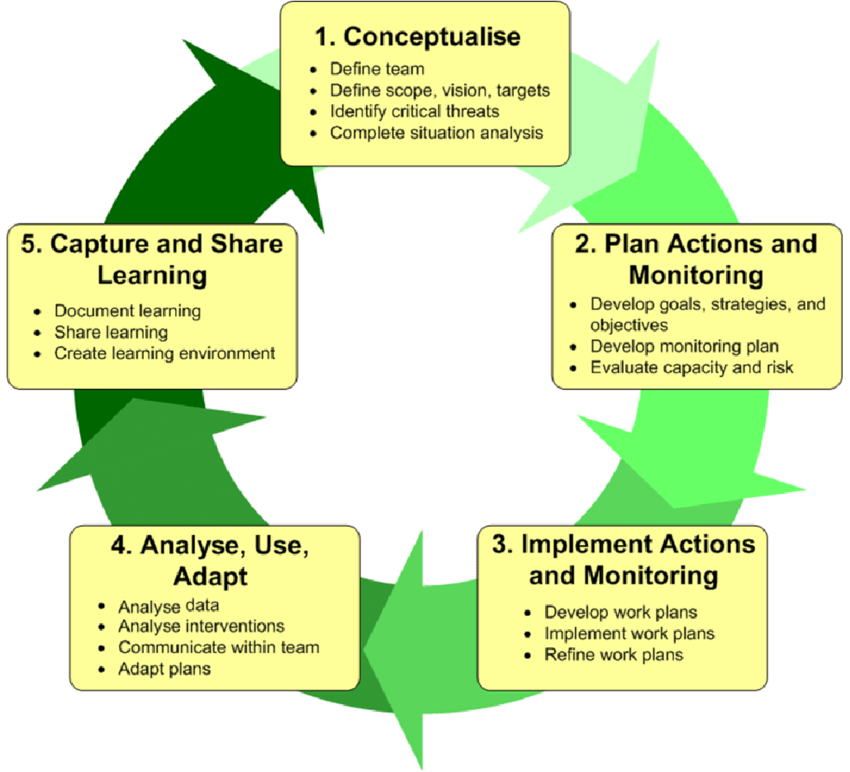
\includegraphics[width=0.75\textwidth]{../figs/The-Open-Standards-adaptive-management-cycle-from-wwwconservationmeasuresorg.png}
 \caption{\textbf{Could we/Do we want to include a version of this Bayesian workflow \citep{gelman2020bayesian} (top panel) or Michael Betancourt's principled Bayesian workflow? Also, it seems aligned with the iterative nature of adaptive management cycles (e.g., bottom panel, from \href{www.conservationmeasures.org}{www.conservationmeasures.org}), which are commonly used in conservation biology. We could consider a 2-paneled figure with something like these? I would like to discuss this as a group, if people think it would be useful}} 
 \label{fig:workflow}
 \end{figure}


\begin{figure}[h]
\centering
 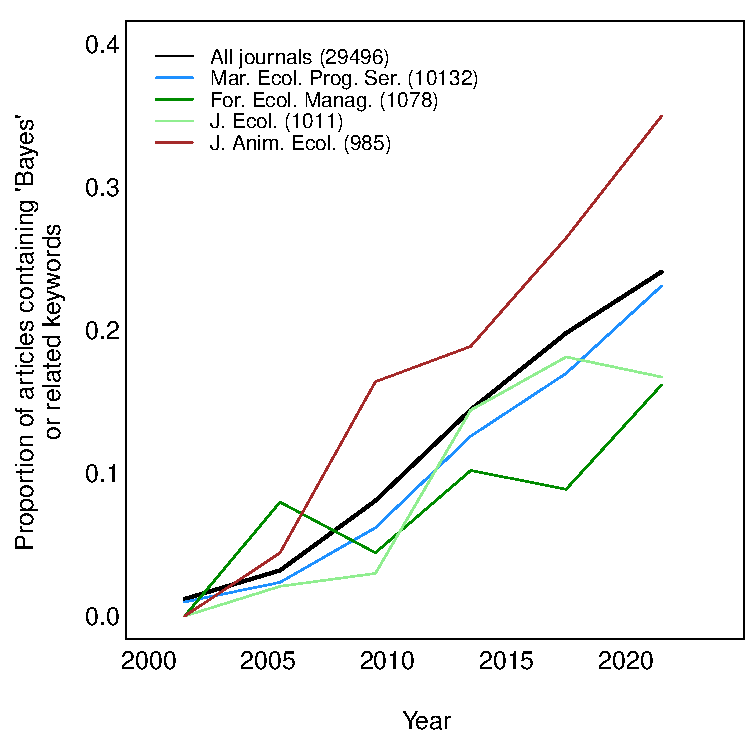
\includegraphics{../figs/conservation.pdf}
 \caption{\textbf{Proportion papers using Bayes in XX major conservation journals since 2000}}
 \label{fig:consbaystrend}
 \end{figure}

%DLJuly30: Still needs an explanation that dashed lines are included for populations with significant growth over time and that in b the points depict the mean change in abundance for each population's posterior estimates and the bars the 90\% uncertainty interval. 
\begin{figure}
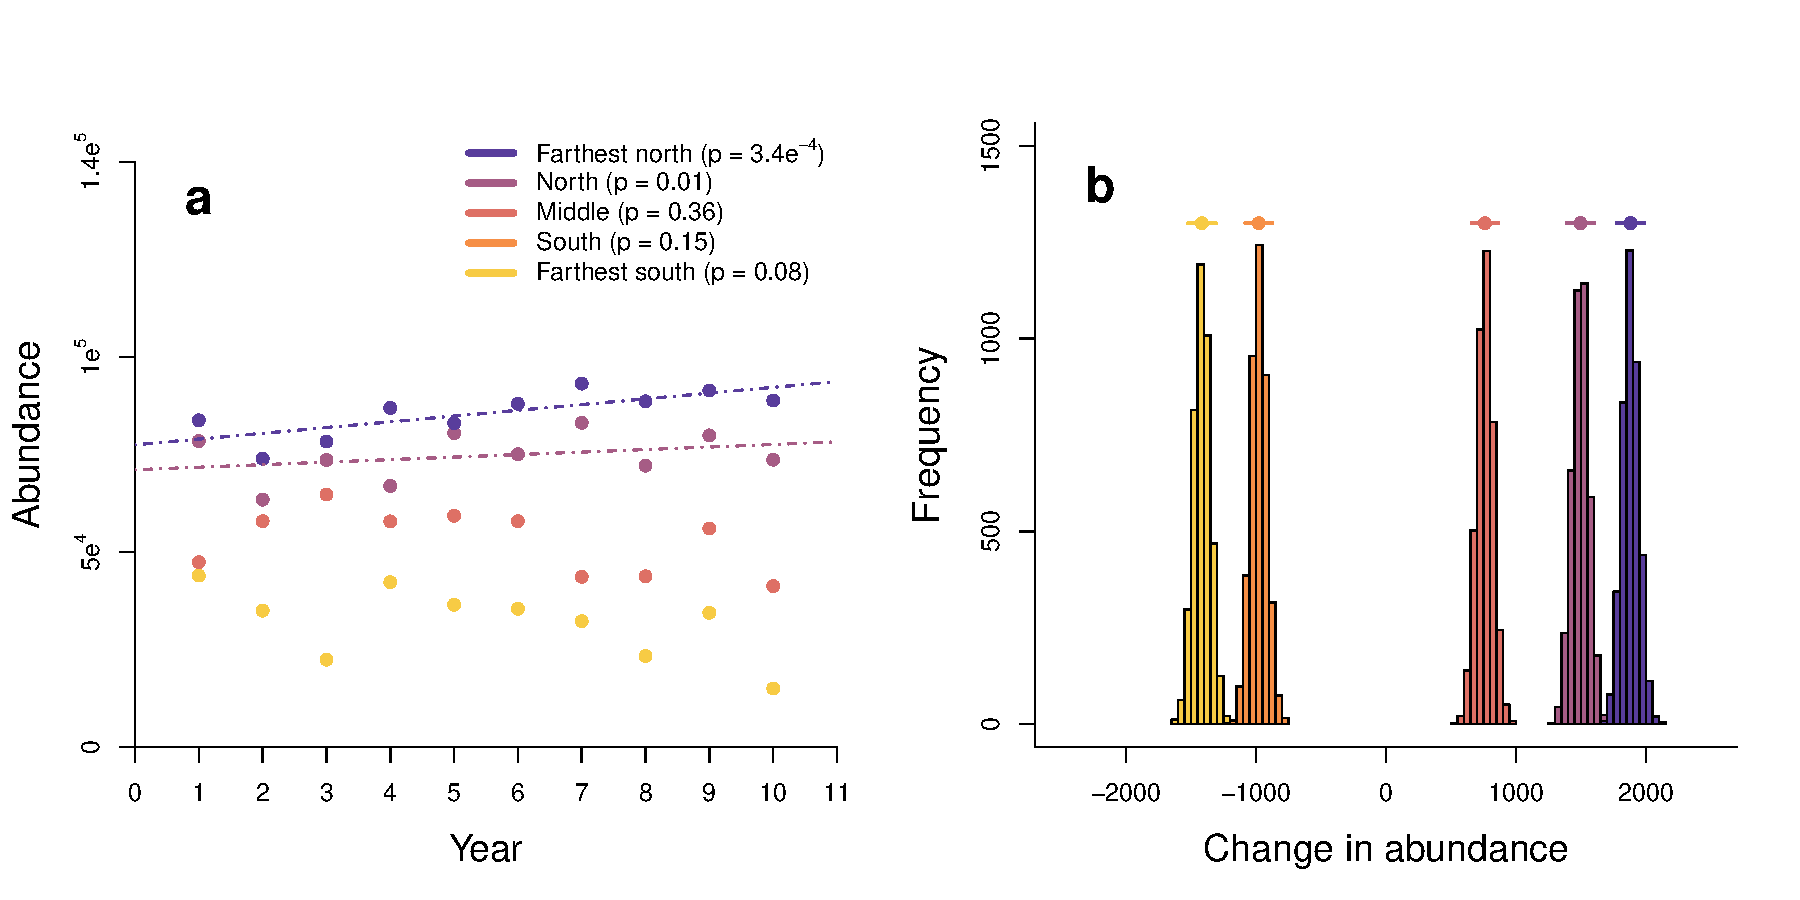
\includegraphics[width=1\textwidth]{../bayesvfisherbox/figures/nhtBoxLayeredMeans.pdf}
\caption{Trends in population size over time (left) analyzed with a traditional Fisherian approach using null hypothesis testing (using an $\alpha$ of 0.05 to reject the null hypothesis of a slope of zero) versus a Bayesian approach, which focuses on the posterior distribution (right).}
\label{fig:nht}
\end{figure}
  %DLJuly30: I would jitter the points to better see the two sets of error
  
 \begin{figure}[h]
\centering
 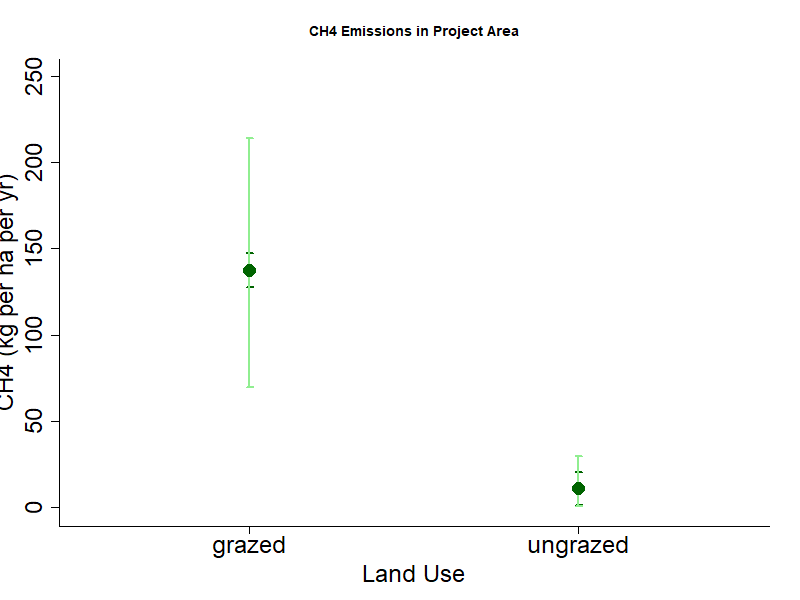
\includegraphics{../figs/ncs/ncsprojimpactch4.png}
 \caption{\textbf{NCS Example: Uncertainty propagation}} 
 \label{fig:ncs}
 \end{figure}
 
 

%%%%%%%%%%%%%%%%%%
%%%%%%%%%%%%%%%%%%%%%%
\end{document}
%%%%%%%%%%%%%%%%%%%%%%%%%%%%%%%%%%%%%%%%
% and for Nationally Determined Contributions, National Adaptation Plans, and other climate plans within the United Nations climate process are informed by the 'best available science.'
%Questions for the group:
%1) How detailed to get in Bayesian methods/theory in introduction?

%Text to add somewhere:
% in the past, climate science and biodiversity fields have been separated, but scientists and decision-makers  are increasingly highlighting  the role nature plays in global climate systems and the critical ecosystem services provided by nature to humans \citep{cohen2016nature,nesshover2017science,USGCRP2024}

